\begin{center}
\bfseries{\large ТЕХНИЧЕСКИЙ ОТЧЁТ ПО ПРАКТИКЕ}
\end{center}

\section*{Архитектура}
У нас есть BD.sm и PrivateBD.sm – это публичная и приватная базы данных, которые записаны в бинарный файл. Там хранятся пары «имя – кодировка лица». 
В файле face\_rec.py находятся функции для работы с базами данных и распознавания лиц.
tg\_bot.py – Телеграм-бот, интерфейс для работы с проектом. Здесь находится логика бота, сам же бот – на серверах Телеграма.
\section*{Описание}
Это Телеграм-бот, который предназначен для распознавания лиц. Для того, чтобы им воспользоваться, необходимо загрузить фотографию человека и подписать её, после чего бот сможет обнаружить этого человека на других фото.
\section*{Реализация}
Создать бота можно через Телеграм-бота @BotFather, там же можно получить токен.
Отправка сообщения на сервер происходит с помощью запроса, направляемого по протоколу HTTP c универсальным идентификатором бота. Ответ обычно приходит в виде объекта формата JSON, где всегда есть булево поле «ok» и (необязательно) поле description строкового типа, где будет описание результатат.

Метод load\_image\_file даёт возможность загрузить фото. Затем обычно используется метод  face\_locations, чтобы определить лицо на фотографии. Далее метод face\_encodings переводит черты лица в где-то 50 вещественных чисел, кодируя его.
Итак, когда требуется уже не добавить лицо в базу данных, а сравнить с уже существующими фото, то вся операция сравнения лиц сводится к сравнению вещественных чисел с определённым шагом «эпсилон» – для большей точности.
И благодаря cv2 мы обводим найденные лица прямоугольниками и подписываем, кто есть кто.
\section*{Тестирование}
Чтобы протестировать бота, в базу данных были добавлены некоторые актёры, а затем отправлялись на распознавание фотографии с этими же актёрами.
Пример работы виден на фото ниже:
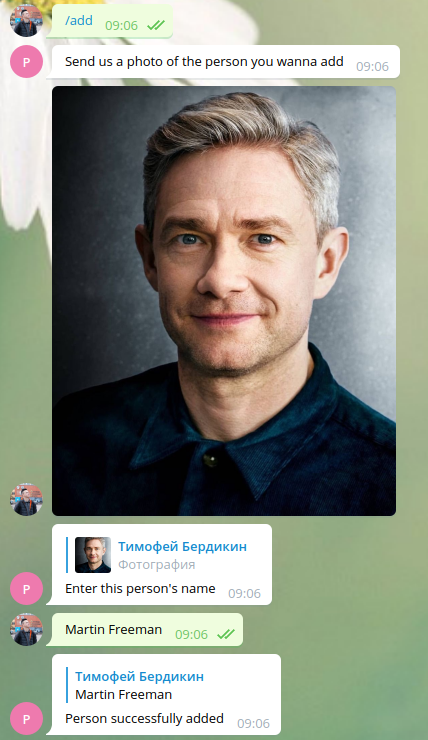
\includegraphics{picture1} \linebreak
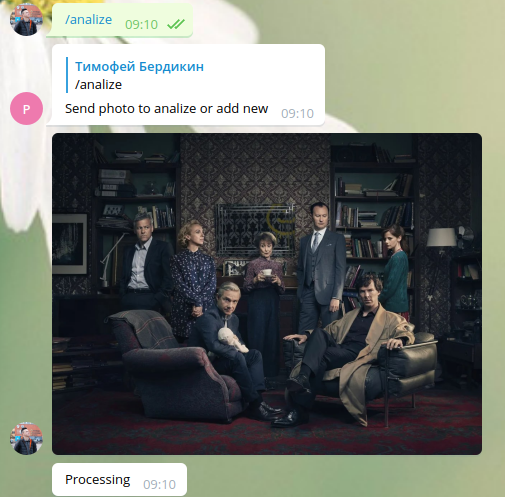
\includegraphics{picture2} \linebreak
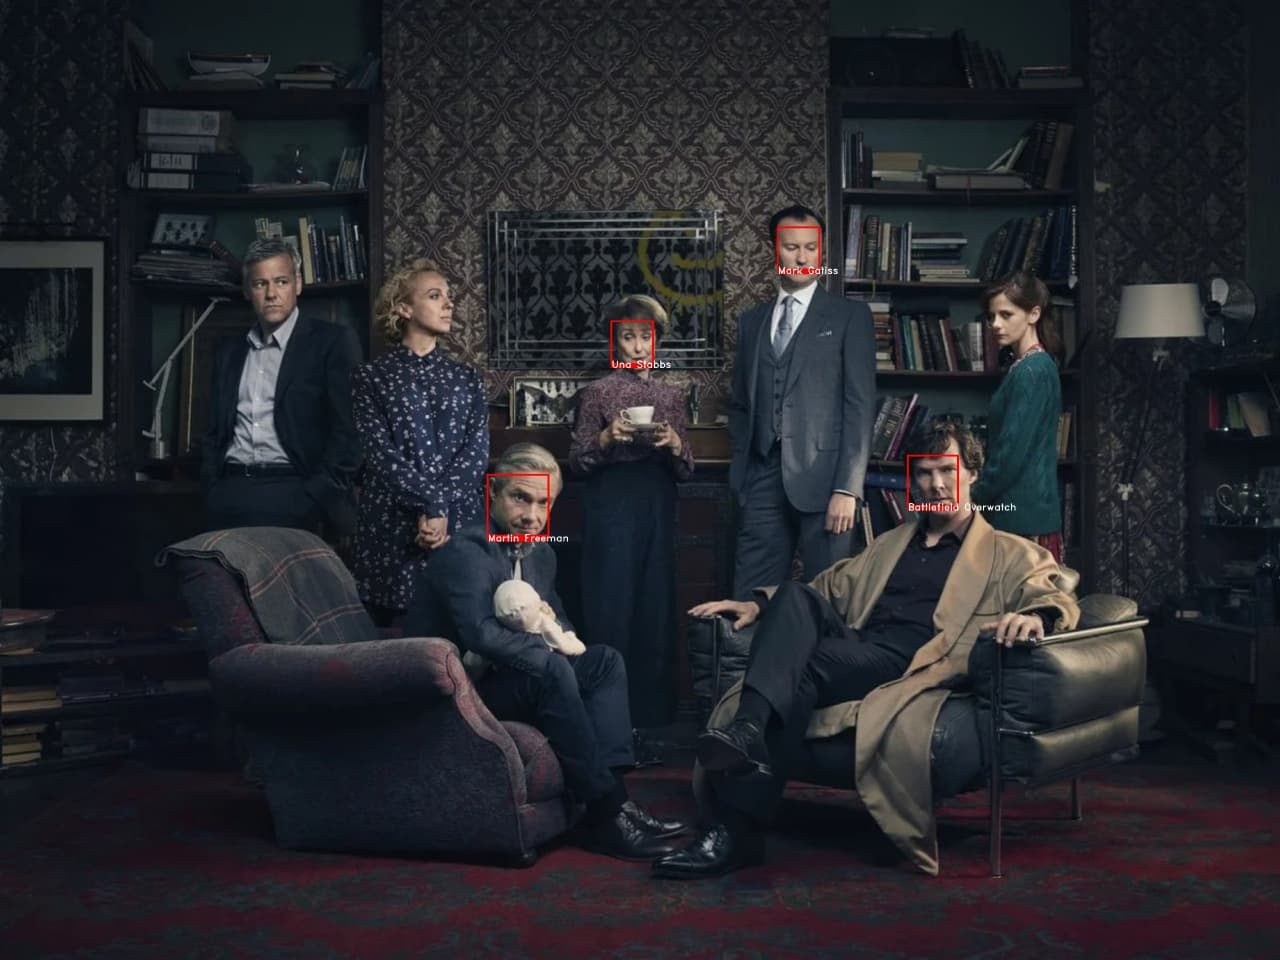
\includegraphics[scale=0.5]{picture3} \linebreak
\section*{Ссылка на GitHub}

\pagebreak
